\section{Lib\-TIM::Flat\-SE Class Reference}
\label{classLibTIM_1_1FlatSE}\index{LibTIM::FlatSE@{LibTIM::FlatSE}}
Container base class for flat structuring elements (or binary masks).  


{\tt \#include $<$Flat\-SE.h$>$}

Inheritance diagram for Lib\-TIM::Flat\-SE::\begin{figure}[H]
\begin{center}
\leavevmode
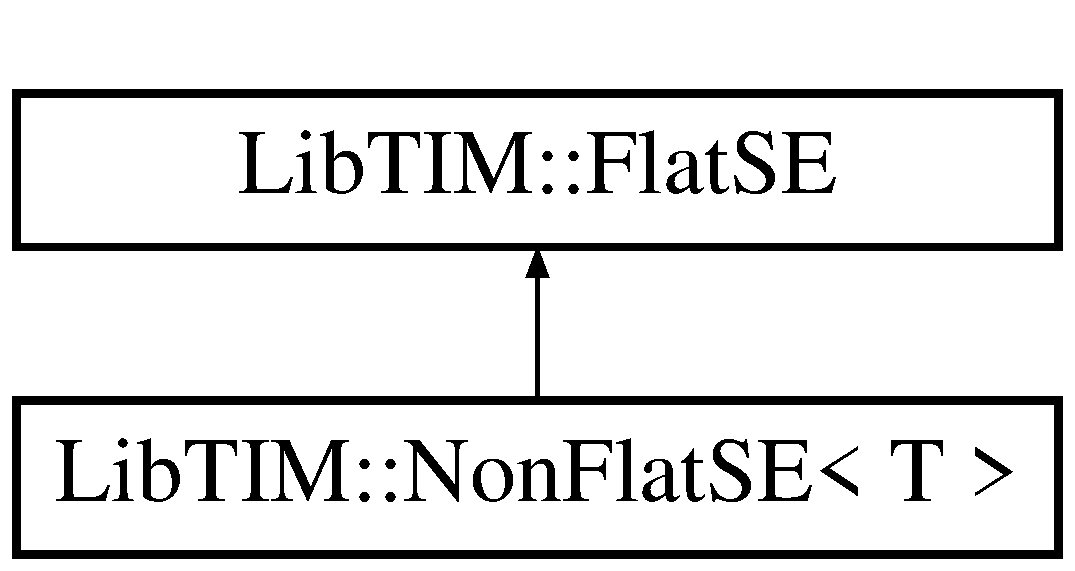
\includegraphics[height=2cm]{classLibTIM_1_1FlatSE}
\end{center}
\end{figure}
\subsection*{Public Types}
\begin{CompactItemize}
\item 
typedef std::vector$<$ {\bf Point}$<$ {\bf TCoord} $>$ $>$::{\bf iterator} {\bf iterator\_\-point}
\item 
typedef std::vector$<$ {\bf TOffset} $>$::{\bf iterator} {\bf iterator\_\-offset}
\item 
typedef {\bf iterator\_\-offset} {\bf iterator}
\end{CompactItemize}
\subsection*{Public Member Functions}
\begin{CompactItemize}
\item 
{\bf Flat\-SE} ()
\item 
{\bf Flat\-SE} (const {\bf Image}$<$ {\bf U8} $>$ \&im)
\item 
{\bf Flat\-SE} \& {\bf Flat\-SE::operator=} (const {\bf Flat\-SE} \&se)
\item 
{\bf Flat\-SE} (const {\bf Flat\-SE} \&se)
\item 
int {\bf get\-Nb\-Points} () const 
\begin{CompactList}\small\item\em returns the number of points contained in the structuring element (cardinal of the set) \item\end{CompactList}\item 
void {\bf set\-Context} (const {\bf TSize} $\ast$size)
\begin{CompactList}\small\item\em computes the offset of each point, according to \char`\"{}size\char`\"{} \item\end{CompactList}\item 
{\bf Point}$<$ {\bf TCoord} $>$ {\bf get\-Point} (int i) const 
\item 
void {\bf add\-Point} ({\bf Point}$<$ {\bf TCoord} $>$ p)
\item 
{\bf TOffset} {\bf get\-Offset} (int point)
\begin{CompactList}\small\item\em returns the offset of \char`\"{}point\char`\"{} \item\end{CompactList}\item 
{\bf TCoord} $\ast$ {\bf get\-Negative\-Offsets} ()
\item 
{\bf TCoord} $\ast$ {\bf get\-Positive\-Offsets} ()
\item 
void {\bf make\-Symmetric} ()
\item 
{\bf Image}$<$ {\bf U8} $>$ {\bf Flat\-SE::to\-Image} ()
\item 
{\bf Flat\-SE} \& {\bf operator+=} ({\bf Flat\-SE} \&b)
\item 
{\bf iterator} {\bf begin} ()
\item 
{\bf iterator} {\bf end} ()
\item 
{\bf iterator\_\-point} {\bf begin\_\-point} ()
\item 
{\bf iterator\_\-point} {\bf end\_\-point} ()
\item 
void {\bf make2DN4} ()
\begin{CompactList}\small\item\em Basic neighborhoods in 2D N4 and N8. \item\end{CompactList}\item 
void {\bf make2DN8} ()
\item 
void {\bf make2DN9} ()
\begin{CompactList}\small\item\em same as before but includes origin \item\end{CompactList}\item 
void {\bf make3DN6} ()
\begin{CompactList}\small\item\em In 3D N6,18,26. \item\end{CompactList}\item 
void {\bf make3DN18} ()
\item 
void {\bf make3DN26} ()
\item 
template$<$class Voxel\-Type$>$ void {\bf make\-Ball\-Euclidian2D} ({\bf Image}$<$ Voxel\-Type $>$ \&img, double r)
\item 
template$<$class Voxel\-Type$>$ void {\bf make\-Ball\-Chessboard2D} ({\bf Image}$<$ Voxel\-Type $>$ \&img, double rx, double ry)
\item 
template$<$class Voxel\-Type$>$ void {\bf make\-Ball\-Euclidian3D} ({\bf Image}$<$ Voxel\-Type $>$ \&img, double r)
\item 
template$<$class Voxel\-Type$>$ void {\bf make\-Circle2D} ({\bf Image}$<$ Voxel\-Type $>$ \&img, double r, double t)
\begin{CompactList}\small\item\em circle with specified thickness \item\end{CompactList}\item 
void {\bf print} ()
\item 
void {\bf reserve} (size\_\-t size)
\item 
void {\bf clear} ()
\end{CompactItemize}
\subsection*{Protected Attributes}
\begin{CompactItemize}
\item 
std::vector$<$ {\bf Point}$<$ {\bf TCoord} $>$ $>$ {\bf points}
\item 
std::vector$<$ {\bf TOffset} $>$ {\bf offsets}
\end{CompactItemize}


\subsection{Detailed Description}
Container base class for flat structuring elements (or binary masks). 

\begin{Desc}
\item[Example:]

\footnotesize\begin{verbatim}	FlatSE se;
	se.make2DN9();
	\end{verbatim}
\normalsize
 creates a 2D structuring element containing a 3x3 square. The origin is at the center. 

\footnotesize\begin{verbatim}	FlatSE se;
	se.makeBallEuclidian2D(r, im);
	\end{verbatim}
\normalsize
 creates 2D structuring element containing a ball of radius r according to the voxels spacing of im. The origin is at the center.\end{Desc}
WARNING: some algorithms require a {\em connexity\/} rather than a structuring element in parameters. To this end, use for example {\bf make2DN8()}{\rm (p.\,\pageref{classLibTIM_1_1FlatSE_a19})} to compute a 8-neighborhood (now the center is {\em not\/} included in the structuring element) Adding a {\em connexity\/} structure is in project.



\subsection{Member Typedef Documentation}
\index{LibTIM::FlatSE@{Lib\-TIM::Flat\-SE}!iterator@{iterator}}
\index{iterator@{iterator}!LibTIM::FlatSE@{Lib\-TIM::Flat\-SE}}
\subsubsection{\setlength{\rightskip}{0pt plus 5cm}typedef {\bf iterator\_\-offset} {\bf Lib\-TIM::Flat\-SE::iterator}}\label{classLibTIM_1_1FlatSE_w2}


\index{LibTIM::FlatSE@{Lib\-TIM::Flat\-SE}!iterator_offset@{iterator\_\-offset}}
\index{iterator_offset@{iterator\_\-offset}!LibTIM::FlatSE@{Lib\-TIM::Flat\-SE}}
\subsubsection{\setlength{\rightskip}{0pt plus 5cm}typedef std::vector$<${\bf TOffset} $>$::{\bf iterator} {\bf Lib\-TIM::Flat\-SE::iterator\_\-offset}}\label{classLibTIM_1_1FlatSE_w1}


\index{LibTIM::FlatSE@{Lib\-TIM::Flat\-SE}!iterator_point@{iterator\_\-point}}
\index{iterator_point@{iterator\_\-point}!LibTIM::FlatSE@{Lib\-TIM::Flat\-SE}}
\subsubsection{\setlength{\rightskip}{0pt plus 5cm}typedef std::vector$<${\bf Point}$<${\bf TCoord}$>$ $>$::{\bf iterator} {\bf Lib\-TIM::Flat\-SE::iterator\_\-point}}\label{classLibTIM_1_1FlatSE_w0}




\subsection{Constructor \& Destructor Documentation}
\index{LibTIM::FlatSE@{Lib\-TIM::Flat\-SE}!FlatSE@{FlatSE}}
\index{FlatSE@{FlatSE}!LibTIM::FlatSE@{Lib\-TIM::Flat\-SE}}
\subsubsection{\setlength{\rightskip}{0pt plus 5cm}Lib\-TIM::Flat\-SE::Flat\-SE ()\hspace{0.3cm}{\tt  [inline]}}\label{classLibTIM_1_1FlatSE_a0}


\index{LibTIM::FlatSE@{Lib\-TIM::Flat\-SE}!FlatSE@{FlatSE}}
\index{FlatSE@{FlatSE}!LibTIM::FlatSE@{Lib\-TIM::Flat\-SE}}
\subsubsection{\setlength{\rightskip}{0pt plus 5cm}Lib\-TIM::Flat\-SE::Flat\-SE (const {\bf Image}$<$ {\bf U8} $>$ \& {\em im})}\label{classLibTIM_1_1FlatSE_a1}


\index{LibTIM::FlatSE@{Lib\-TIM::Flat\-SE}!FlatSE@{FlatSE}}
\index{FlatSE@{FlatSE}!LibTIM::FlatSE@{Lib\-TIM::Flat\-SE}}
\subsubsection{\setlength{\rightskip}{0pt plus 5cm}Lib\-TIM::Flat\-SE::Flat\-SE (const {\bf Flat\-SE} \& {\em se})\hspace{0.3cm}{\tt  [inline]}}\label{classLibTIM_1_1FlatSE_a3}




\subsection{Member Function Documentation}
\index{LibTIM::FlatSE@{Lib\-TIM::Flat\-SE}!addPoint@{addPoint}}
\index{addPoint@{addPoint}!LibTIM::FlatSE@{Lib\-TIM::Flat\-SE}}
\subsubsection{\setlength{\rightskip}{0pt plus 5cm}void Lib\-TIM::Flat\-SE::add\-Point ({\bf Point}$<$ {\bf TCoord} $>$ {\em p})\hspace{0.3cm}{\tt  [inline]}}\label{classLibTIM_1_1FlatSE_a7}


\index{LibTIM::FlatSE@{Lib\-TIM::Flat\-SE}!begin@{begin}}
\index{begin@{begin}!LibTIM::FlatSE@{Lib\-TIM::Flat\-SE}}
\subsubsection{\setlength{\rightskip}{0pt plus 5cm}{\bf iterator} Lib\-TIM::Flat\-SE::begin ()\hspace{0.3cm}{\tt  [inline]}}\label{classLibTIM_1_1FlatSE_a14}


\index{LibTIM::FlatSE@{Lib\-TIM::Flat\-SE}!begin_point@{begin\_\-point}}
\index{begin_point@{begin\_\-point}!LibTIM::FlatSE@{Lib\-TIM::Flat\-SE}}
\subsubsection{\setlength{\rightskip}{0pt plus 5cm}{\bf iterator\_\-point} Lib\-TIM::Flat\-SE::begin\_\-point ()\hspace{0.3cm}{\tt  [inline]}}\label{classLibTIM_1_1FlatSE_a16}


\index{LibTIM::FlatSE@{Lib\-TIM::Flat\-SE}!clear@{clear}}
\index{clear@{clear}!LibTIM::FlatSE@{Lib\-TIM::Flat\-SE}}
\subsubsection{\setlength{\rightskip}{0pt plus 5cm}void Lib\-TIM::Flat\-SE::clear ()\hspace{0.3cm}{\tt  [inline]}}\label{classLibTIM_1_1FlatSE_a30}




Reimplemented in {\bf Lib\-TIM::Non\-Flat\-SE$<$ T $>$} {\rm (p.\,\pageref{classLibTIM_1_1NonFlatSE_a10})}.\index{LibTIM::FlatSE@{Lib\-TIM::Flat\-SE}!end@{end}}
\index{end@{end}!LibTIM::FlatSE@{Lib\-TIM::Flat\-SE}}
\subsubsection{\setlength{\rightskip}{0pt plus 5cm}{\bf iterator} Lib\-TIM::Flat\-SE::end ()\hspace{0.3cm}{\tt  [inline]}}\label{classLibTIM_1_1FlatSE_a15}


\index{LibTIM::FlatSE@{Lib\-TIM::Flat\-SE}!end_point@{end\_\-point}}
\index{end_point@{end\_\-point}!LibTIM::FlatSE@{Lib\-TIM::Flat\-SE}}
\subsubsection{\setlength{\rightskip}{0pt plus 5cm}{\bf iterator\_\-point} Lib\-TIM::Flat\-SE::end\_\-point ()\hspace{0.3cm}{\tt  [inline]}}\label{classLibTIM_1_1FlatSE_a17}


\index{LibTIM::FlatSE@{Lib\-TIM::Flat\-SE}!FlatSE::operator=@{FlatSE::operator=}}
\index{FlatSE::operator=@{FlatSE::operator=}!LibTIM::FlatSE@{Lib\-TIM::Flat\-SE}}
\subsubsection{\setlength{\rightskip}{0pt plus 5cm}{\bf Flat\-SE}\& Lib\-TIM::Flat\-SE::Flat\-SE::operator= (const {\bf Flat\-SE} \& {\em se})}\label{classLibTIM_1_1FlatSE_a2}


\index{LibTIM::FlatSE@{Lib\-TIM::Flat\-SE}!FlatSE::toImage@{FlatSE::toImage}}
\index{FlatSE::toImage@{FlatSE::toImage}!LibTIM::FlatSE@{Lib\-TIM::Flat\-SE}}
\subsubsection{\setlength{\rightskip}{0pt plus 5cm}{\bf Image}$<${\bf U8}$>$ Lib\-TIM::Flat\-SE::Flat\-SE::to\-Image ()}\label{classLibTIM_1_1FlatSE_a12}


\index{LibTIM::FlatSE@{Lib\-TIM::Flat\-SE}!getNbPoints@{getNbPoints}}
\index{getNbPoints@{getNbPoints}!LibTIM::FlatSE@{Lib\-TIM::Flat\-SE}}
\subsubsection{\setlength{\rightskip}{0pt plus 5cm}int Lib\-TIM::Flat\-SE::get\-Nb\-Points () const\hspace{0.3cm}{\tt  [inline]}}\label{classLibTIM_1_1FlatSE_a4}


returns the number of points contained in the structuring element (cardinal of the set) 

\index{LibTIM::FlatSE@{Lib\-TIM::Flat\-SE}!getNegativeOffsets@{getNegativeOffsets}}
\index{getNegativeOffsets@{getNegativeOffsets}!LibTIM::FlatSE@{Lib\-TIM::Flat\-SE}}
\subsubsection{\setlength{\rightskip}{0pt plus 5cm}{\bf TCoord} $\ast$ Lib\-TIM::Flat\-SE::get\-Negative\-Offsets ()\hspace{0.3cm}{\tt  [inline]}}\label{classLibTIM_1_1FlatSE_a9}


\index{LibTIM::FlatSE@{Lib\-TIM::Flat\-SE}!getOffset@{getOffset}}
\index{getOffset@{getOffset}!LibTIM::FlatSE@{Lib\-TIM::Flat\-SE}}
\subsubsection{\setlength{\rightskip}{0pt plus 5cm}{\bf TOffset} Lib\-TIM::Flat\-SE::get\-Offset (int {\em point})\hspace{0.3cm}{\tt  [inline]}}\label{classLibTIM_1_1FlatSE_a8}


returns the offset of \char`\"{}point\char`\"{} 

\index{LibTIM::FlatSE@{Lib\-TIM::Flat\-SE}!getPoint@{getPoint}}
\index{getPoint@{getPoint}!LibTIM::FlatSE@{Lib\-TIM::Flat\-SE}}
\subsubsection{\setlength{\rightskip}{0pt plus 5cm}{\bf Point}$<${\bf TCoord}$>$ Lib\-TIM::Flat\-SE::get\-Point (int {\em i}) const\hspace{0.3cm}{\tt  [inline]}}\label{classLibTIM_1_1FlatSE_a6}


\index{LibTIM::FlatSE@{Lib\-TIM::Flat\-SE}!getPositiveOffsets@{getPositiveOffsets}}
\index{getPositiveOffsets@{getPositiveOffsets}!LibTIM::FlatSE@{Lib\-TIM::Flat\-SE}}
\subsubsection{\setlength{\rightskip}{0pt plus 5cm}{\bf TCoord} $\ast$ Lib\-TIM::Flat\-SE::get\-Positive\-Offsets ()\hspace{0.3cm}{\tt  [inline]}}\label{classLibTIM_1_1FlatSE_a10}


\index{LibTIM::FlatSE@{Lib\-TIM::Flat\-SE}!make2DN4@{make2DN4}}
\index{make2DN4@{make2DN4}!LibTIM::FlatSE@{Lib\-TIM::Flat\-SE}}
\subsubsection{\setlength{\rightskip}{0pt plus 5cm}void Lib\-TIM::Flat\-SE::make2DN4 ()\hspace{0.3cm}{\tt  [inline]}}\label{classLibTIM_1_1FlatSE_a18}


Basic neighborhoods in 2D N4 and N8. 

Basic neighborhood (4-neighborhood). Warning: do not contain the origin!\index{LibTIM::FlatSE@{Lib\-TIM::Flat\-SE}!make2DN8@{make2DN8}}
\index{make2DN8@{make2DN8}!LibTIM::FlatSE@{Lib\-TIM::Flat\-SE}}
\subsubsection{\setlength{\rightskip}{0pt plus 5cm}void Lib\-TIM::Flat\-SE::make2DN8 ()\hspace{0.3cm}{\tt  [inline]}}\label{classLibTIM_1_1FlatSE_a19}


Basic neighborhood (8-neighborhood). Warning: do not contain the origin!\index{LibTIM::FlatSE@{Lib\-TIM::Flat\-SE}!make2DN9@{make2DN9}}
\index{make2DN9@{make2DN9}!LibTIM::FlatSE@{Lib\-TIM::Flat\-SE}}
\subsubsection{\setlength{\rightskip}{0pt plus 5cm}void Lib\-TIM::Flat\-SE::make2DN9 ()\hspace{0.3cm}{\tt  [inline]}}\label{classLibTIM_1_1FlatSE_a20}


same as before but includes origin 

\index{LibTIM::FlatSE@{Lib\-TIM::Flat\-SE}!make3DN18@{make3DN18}}
\index{make3DN18@{make3DN18}!LibTIM::FlatSE@{Lib\-TIM::Flat\-SE}}
\subsubsection{\setlength{\rightskip}{0pt plus 5cm}void Lib\-TIM::Flat\-SE::make3DN18 ()}\label{classLibTIM_1_1FlatSE_a22}


\index{LibTIM::FlatSE@{Lib\-TIM::Flat\-SE}!make3DN26@{make3DN26}}
\index{make3DN26@{make3DN26}!LibTIM::FlatSE@{Lib\-TIM::Flat\-SE}}
\subsubsection{\setlength{\rightskip}{0pt plus 5cm}void Lib\-TIM::Flat\-SE::make3DN26 ()}\label{classLibTIM_1_1FlatSE_a23}


\index{LibTIM::FlatSE@{Lib\-TIM::Flat\-SE}!make3DN6@{make3DN6}}
\index{make3DN6@{make3DN6}!LibTIM::FlatSE@{Lib\-TIM::Flat\-SE}}
\subsubsection{\setlength{\rightskip}{0pt plus 5cm}void Lib\-TIM::Flat\-SE::make3DN6 ()}\label{classLibTIM_1_1FlatSE_a21}


In 3D N6,18,26. 

\index{LibTIM::FlatSE@{Lib\-TIM::Flat\-SE}!makeBallChessboard2D@{makeBallChessboard2D}}
\index{makeBallChessboard2D@{makeBallChessboard2D}!LibTIM::FlatSE@{Lib\-TIM::Flat\-SE}}
\subsubsection{\setlength{\rightskip}{0pt plus 5cm}template$<$class Voxel\-Type$>$ void Lib\-TIM::Flat\-SE::make\-Ball\-Chessboard2D ({\bf Image}$<$ Voxel\-Type $>$ \& {\em img}, double {\em rx}, double {\em ry})}\label{classLibTIM_1_1FlatSE_a25}


\index{LibTIM::FlatSE@{Lib\-TIM::Flat\-SE}!makeBallEuclidian2D@{makeBallEuclidian2D}}
\index{makeBallEuclidian2D@{makeBallEuclidian2D}!LibTIM::FlatSE@{Lib\-TIM::Flat\-SE}}
\subsubsection{\setlength{\rightskip}{0pt plus 5cm}template$<$class Voxel\-Type$>$ void Lib\-TIM::Flat\-SE::make\-Ball\-Euclidian2D ({\bf Image}$<$ Voxel\-Type $>$ \& {\em img}, double {\em r})}\label{classLibTIM_1_1FlatSE_a24}


\index{LibTIM::FlatSE@{Lib\-TIM::Flat\-SE}!makeBallEuclidian3D@{makeBallEuclidian3D}}
\index{makeBallEuclidian3D@{makeBallEuclidian3D}!LibTIM::FlatSE@{Lib\-TIM::Flat\-SE}}
\subsubsection{\setlength{\rightskip}{0pt plus 5cm}template$<$class Voxel\-Type$>$ void Lib\-TIM::Flat\-SE::make\-Ball\-Euclidian3D ({\bf Image}$<$ Voxel\-Type $>$ \& {\em img}, double {\em r})}\label{classLibTIM_1_1FlatSE_a26}


\index{LibTIM::FlatSE@{Lib\-TIM::Flat\-SE}!makeCircle2D@{makeCircle2D}}
\index{makeCircle2D@{makeCircle2D}!LibTIM::FlatSE@{Lib\-TIM::Flat\-SE}}
\subsubsection{\setlength{\rightskip}{0pt plus 5cm}template$<$class T$>$ void Lib\-TIM::Flat\-SE::make\-Circle2D ({\bf Image}$<$ Voxel\-Type $>$ \& {\em img}, double {\em r}, double {\em t})}\label{classLibTIM_1_1FlatSE_a27}


circle with specified thickness 

\index{LibTIM::FlatSE@{Lib\-TIM::Flat\-SE}!makeSymmetric@{makeSymmetric}}
\index{makeSymmetric@{makeSymmetric}!LibTIM::FlatSE@{Lib\-TIM::Flat\-SE}}
\subsubsection{\setlength{\rightskip}{0pt plus 5cm}void Lib\-TIM::Flat\-SE::make\-Symmetric ()\hspace{0.3cm}{\tt  [inline]}}\label{classLibTIM_1_1FlatSE_a11}


\index{LibTIM::FlatSE@{Lib\-TIM::Flat\-SE}!operator+=@{operator+=}}
\index{operator+=@{operator+=}!LibTIM::FlatSE@{Lib\-TIM::Flat\-SE}}
\subsubsection{\setlength{\rightskip}{0pt plus 5cm}{\bf Flat\-SE}\& Lib\-TIM::Flat\-SE::operator+= ({\bf Flat\-SE} \& {\em b})\hspace{0.3cm}{\tt  [inline]}}\label{classLibTIM_1_1FlatSE_a13}


\index{LibTIM::FlatSE@{Lib\-TIM::Flat\-SE}!print@{print}}
\index{print@{print}!LibTIM::FlatSE@{Lib\-TIM::Flat\-SE}}
\subsubsection{\setlength{\rightskip}{0pt plus 5cm}void Lib\-TIM::Flat\-SE::print ()\hspace{0.3cm}{\tt  [inline]}}\label{classLibTIM_1_1FlatSE_a28}




Reimplemented in {\bf Lib\-TIM::Non\-Flat\-SE$<$ T $>$} {\rm (p.\,\pageref{classLibTIM_1_1NonFlatSE_a8})}.\index{LibTIM::FlatSE@{Lib\-TIM::Flat\-SE}!reserve@{reserve}}
\index{reserve@{reserve}!LibTIM::FlatSE@{Lib\-TIM::Flat\-SE}}
\subsubsection{\setlength{\rightskip}{0pt plus 5cm}void Lib\-TIM::Flat\-SE::reserve (size\_\-t {\em size})\hspace{0.3cm}{\tt  [inline]}}\label{classLibTIM_1_1FlatSE_a29}




Reimplemented in {\bf Lib\-TIM::Non\-Flat\-SE$<$ T $>$} {\rm (p.\,\pageref{classLibTIM_1_1NonFlatSE_a9})}.\index{LibTIM::FlatSE@{Lib\-TIM::Flat\-SE}!setContext@{setContext}}
\index{setContext@{setContext}!LibTIM::FlatSE@{Lib\-TIM::Flat\-SE}}
\subsubsection{\setlength{\rightskip}{0pt plus 5cm}void Lib\-TIM::Flat\-SE::set\-Context (const {\bf TSize} $\ast$ {\em size})\hspace{0.3cm}{\tt  [inline]}}\label{classLibTIM_1_1FlatSE_a5}


computes the offset of each point, according to \char`\"{}size\char`\"{} 



\subsection{Member Data Documentation}
\index{LibTIM::FlatSE@{Lib\-TIM::Flat\-SE}!offsets@{offsets}}
\index{offsets@{offsets}!LibTIM::FlatSE@{Lib\-TIM::Flat\-SE}}
\subsubsection{\setlength{\rightskip}{0pt plus 5cm}std::vector$<${\bf TOffset}$>$ {\bf Lib\-TIM::Flat\-SE::offsets}\hspace{0.3cm}{\tt  [protected]}}\label{classLibTIM_1_1FlatSE_p1}


\index{LibTIM::FlatSE@{Lib\-TIM::Flat\-SE}!points@{points}}
\index{points@{points}!LibTIM::FlatSE@{Lib\-TIM::Flat\-SE}}
\subsubsection{\setlength{\rightskip}{0pt plus 5cm}std::vector$<${\bf Point}$<${\bf TCoord}$>$ $>$ {\bf Lib\-TIM::Flat\-SE::points}\hspace{0.3cm}{\tt  [protected]}}\label{classLibTIM_1_1FlatSE_p0}




The documentation for this class was generated from the following files:\begin{CompactItemize}
\item 
Common/{\bf Flat\-SE.h}\item 
Common/{\bf Flat\-SE.hxx}\end{CompactItemize}
